% Copyright 2021 Jacopo Maltagliati
%
% Use of this source code is governed by an EUPL-style
% license that can be found in the LICENSE file or at
% https://eupl.eu/1.2/en/.
% A localized copy of this license can be found in the LICENSE.it file or at
% https://eupl.eu/1.2/it/
%
% Portions of this document are subject to different licensing agreements,
% see src/titlepage.tex for details.

\documentclass[a4paper,12pt]{report}
\usepackage[paper=a4paper,margin=1in]{geometry}
\usepackage{graphicx}
\usepackage{float}
%\usepackage{hyperref}
\usepackage[T1]{fontenc}
\usepackage{lmodern}
\usepackage[utf8]{inputenc}
\usepackage{setspace}
\usepackage[english]{babel}
%\usepackage{amssymb}
%\usepackage{amsthm}
%\usepackage{amsmath}
%\usepackage{amstext}
\usepackage{microtype}
\usepackage{csquotes}
\usepackage{bookmark}
\usepackage{xpatch}
\usepackage{listings}
\usepackage{minted}
\usemintedstyle{borland}
\usepackage[backend=biber, sorting=none]{biblatex}
\hypersetup{colorlinks=true, linkcolor=blue, citecolor=blue, urlcolor=blue, pdftitle={Linux as a Real-Time Operating System}}
\addbibresource{all.bib}
\usepackage[color=green,textsize=tiny]{todonotes}
\newcommand{\xxx}[1]{\todo[color=red]{#1}}
\usepackage{sectsty}
\chapternumberfont{\large}
\chaptertitlefont{\huge}
\renewcommand{\familydefault}{\sfdefault}
\newcommand{\comment}[1]{}
\begin{document}
% Titlepage
% Copyright 2020 Luca Chiodini
%
% Use of this source code is governed by an MIT-style
% license that can be found in the LICENSE file or at
% https://opensource.org/licenses/MIT.
%
% The Università degli Studi di Milano-Bicocca "ottaedro leonardesco" logo is
% protected by copyright, and it can be used under the terms and conditions
% that can be found in the logo-license.pdf file, or at
% https://www.unimib.it/sites/default/files/Allegati/regolamento.pdf.

\begin{titlepage}

    \noindent
    \begin{minipage}[t]{0.19\textwidth}
        \vspace{-4mm}{\includegraphics[scale=1.15]{logo.pdf}}
    \end{minipage}
    \begin{minipage}[t]{0.81\textwidth}
        {
            \setstretch{1.42}
            {\textsc{Università degli Studi di Milano - Bicocca}} \\
            \textbf{Scuola di Scienze} \\
            \textbf{Dipartimento di Informatica, Sistemistica e Comunicazione} \\
            \textbf{Corso di laurea in Informatica} \\
            \par
        }
    \end{minipage}

    \vspace{35mm}

    \begin{center}
        {\Huge{
                \setstretch{1.2}
                \textbf{Linux as a Real-Time Operating System: a practical analysis in the mobile robotics domain}
                \par
            }
        }
    \end{center}

    \vspace{30mm}

    \noindent
    {\large \textbf{Relatore:} Prof. Sorrenti Domenico } \\

    \noindent
    {\large \textbf{Co-relatore:} Prof. Braione Pietro } \\
    
    \noindent
    {\large \textbf{Co-relatore:} Prof. Ferretti Claudio }

    \vspace{15mm}

    \begin{flushright}
        {\large \textbf{Relazione della prova finale di:}} \\
        \large{Jacopo Maltagliati} \\
        \large{Matricola 830110}
    \end{flushright}

    \vspace{2mm}

    \begin{center}
        {\large{\bf Anno Accademico 2019-2020}}
    \end{center}

    \restoregeometry

\end{titlepage}
\newpage
% Quote
\vspace*{\stretch{1}}
\begin{flushright}
  \itshape
  \begin{tabular}{@{}l@{}}
    In (conflicted) memory\\of Viale Fulvio Testi 174\\
    2017-2020\\JM,MP,MS,MT,AM,MC 
  \end{tabular}
\end{flushright}
\vspace{\stretch{2}}
\newpage
% Toc
\tableofcontents
\newpage
% Set paragraph spacing so our eyes don't pop while reading
\setlength{\parskip}{1em}
% Ch0
\chapter*{Acknowledgements}
A special thanks for the continued support and previous work on Otto, ROS and the USAD platform goes to Domenico Sorrenti, Federica Di Lauro, Simone Fontana, Carlo Radice, Giovanni Capra and Riccardo Curnis of the IRAlab team, and to the former IRAlab member Augusto Luis Ballardini.

% Ch1
\chapter{Summary}

In the past decade, mobile robotics as a field has been gaining a lot of traction: as technology evolves, building a mobile platform has become more and more feasible for anyone, including small research teams and hobbyists. The GNU/Linux operating system is a perfect starting point for these people, being a mature and constantly evolving environment that includes powerful development tools and the complete source code out of the box, free of charge.

However, there is still a lack of easily approachable real-time solutions able to manage the workload, as many of the available frameworks are not mature enough to offer fine-grained real time application control: this is why we ultimately decided to push the Linux kernel to its limits, studying its real-time capabilities and ease of use.

\section{The problem}

Imagine driving on an empty road at night while listening to classical music: it's been a very long day, and your consciousness gradually drifts to a peaceful slumber. Suddenly, an animal crosses the road: are you going to notice? Will you be able to stop in time? Now, consider a self-driving car in the same situation: what would happen if the control computer "dozed off" even for a fraction of a second? The user would probably not be able to stomp on the brakes fast enough to prevent the car from crashing.

A possible solution to this problem is carefully designing a system built around existing technologies, such as real-time control, redundant hardware platforms, and failsafe mechanisms. However, creating a real-time system from the ground up tends to be very expensive and error-prone, as incorrect design or minor mistakes could lead to catastrophic failures such as the infamous Therac-25 \cite{therac-25-accidents} incident.

For this reason, many software houses have been working on various commercial solutions since the 1980s that enabled programmers and engineers to deploy their application on proven grounds, thus reducing the time and effort needed to create a real-time application. Arguably, the best aspect of those systems was their widespread availability: for example, DEC's VAXeln used lightly modified VAX computers, and Quantum Computer Inc. QNX ran on consumer-grade hardware, including x86 processors. While the VAXeln is now a historical platform, QNX is still commercially available from BlackBerry Limited and major companies such as Apple use it for their products \cite{time-carplay-qnx}.

However, having always demonstrated incredible versability, the ubiquitous Linux kernel is becoming a viable option for robotics and real-time usage, with both academic and commercial applications exploiting it like Tesla Motors, which maintains its own fork \cite{gh-tesla-linux}. Of course, flexibility comes at the cost of reduced effectiveness in each specific situation, so why do many endeavors use Linux? Possibly because:
\begin{itemize}
  \item Most Linux distributions come completely free of charge, so even low-budget organizations can afford to use them.
  \item The Linux kernel and the GNU userland are open-source and can be modified to meet specific needs by people with the right expertise.
  \item The Linux ecosystem has a wide community of developers who are constantly improving it, ensuring constant maintenance and security updates even for organizations without any support contract.
  \item Linux provides a full development environment out-of-the-box, something that we may take for granted nowadays but is still a costly optional feature on many systems.
\end{itemize}

These, along with the fact that IRAlab has already been running Linux on their platforms for several years, are the reasons why we decided to adopt it for this project.

\section{Current implementation}

At the moment, most of IRAlab's mobile platforms are controlled by a master node running Ubuntu Linux 16.04 LTS and the ROS framework, which was created by Willow Garage as a rapid development platform for their PR2 robot and traces its roots into an even earlier effort by a team of researchers and students at Stanford University. 

The name "Robot Operating System" is misleading: in fact, ROS is mostly an open-source middleware, that is a set of software libraries and tools that help you build robot applications, which needs an underlying operating system to run: currently, it may do so on both Unix-like operating systems such as Ubuntu GNU/Linux, BlackBerry QNX \cite{qnx-ros} and Apple macOS, and on some Microsoft Windows versions. For simplicity, we'll use the term "ROS" to refer to the ROS+Linux combination throughout this report.

\subsection{Description}

Currently, IRAlab mainly uses a customized ROS navigation stack for abstraction and rapid prototyping: through the use of \textit{topics} and \textit{messages}, ROS provides a facility to let the users write small programs, called \textit{nodes}, and make them communicate with each other. A \textit{master node}, provided by the framework, acts as a central hub, keeping tabs on the state of the \textit{Computational Graph}. Moreover, ROS provides extensive \textit{timestamping} and data logging facilities, letting the user easily track, monitor, and simulate a mobile platform's behavior.

An in-depth analysis of the ROS functionalities and usage in the context of our mobile platforms is beyond the scope of this report, but it has received extensive coverage in earlier works performed by IRAlab members, such as \textcite{fdila-bs-otto}.

\subsection{Issues}

The problem we encountered with ROS is its complexity: while it's easily modifiable and extensible, there is no simple way to control precisely how the nodes are scheduled. Finely tuning this behavior would imply heavily modifying the codebase, which is a very complex task.

Ultimately, some parts of ROS are written in Python \cite{roswiki-rospy} which is, in its CPython implementation, an interpreted language. Python is notoriously hard to control in a real-time environment since it uses facilities like garbage collection \cite{python-devguide-gc} and dynamic allocation that are not designed to obey real-time constraints. The easiest way to avoid this problem is to use a language such as C, which gives the programmer more control over the timing and scheduling of the threads.

An attempt to solve this problem has been made by \textcite{rt-ros-approach}: by using a co-kernel approach, the authors moved some of the ROS nodes to a second processing unit and ran them as real-time tasks on the NuttX microkernel. For our goals, though, we've deemed it as an unnecessarily complex workaround and decided to explore different solutions.

\section{A possible upgrade path}

To develop a complex application cost-effectively, using some scaffolding is necessary to avoid spending more time designing your software than implementing it: this is why the ROS framework, which doubles as a rapid prototyping platform, has gained so much traction in the last decade. 

However, there are several common pitfalls associated with them: increasing modularity inevitably leads to more complex runtimes that must be bundled with your application and cannot be easily modified. While a modular design should address this problem, a fundamental design decision taken by the developers of the framework that clashes with the needs of your application would force you to move to a different platform entirely.

It's impossible to know whether or not such a solution would be suitable for your application beforehand without doing some research: this is why we've decided to study the innards of the ROS 2 framework, which seemed like a viable upgrade path.

\subsubsection{Robot Operating System, version 2}

ROS 2, the new generation of the ROS platform, was launched in 2015 and has reached its seventh release, and was subject to a complete redesign revolving around an enterprise-grade communications subsystem that is much more RT-friendly \cite{dds-design-performance}, in an attempt to solve the shortcomings of ROS \cite{ros2-realtime-intro}. 

Initially, we hoped that using this framework would've enabled us to benefit from the new real-time design without the burden of porting our navigation stack to an entirely new platform: this would've reduced turnaround time significantly, and let us focus more on tuning the performance of the system.

However, before we could evaluate those benefits, we determined that adopting ROS 2 would not be a wise choice since its architecture makes it impossible for the programmer to precisely control the timing of a specific portion of code within a task with an RT-scheduler provided by Linux such as \texttt{RT} or \texttt{DEADLINE}. Specifically, the task pipeline in ROS 2 uses one or more "super-threads" inside of which a custom scheduling algorithm is in charge of scheduling a variable number of tasks\cite{ros2-rt-analysis}: while this design is more real-time friendly than its predecessor's, it's ultimately even more opaque to the underlying operating system, and thus to the programmer, than the previous one.

\newpage
% Ch2
\chapter{Solution}

Our custom solution, named \texttt{rt-app}, is a demonstration of what we believe is a viable approach for building real-time control systems on Linux. Written from scratch, the demo currently leverages several APIs provided by Linux such as \texttt{sched(7)} \cite{man-sched-7}, \texttt{time(7)} \cite{man-time-7} and \texttt{pthreads(7)} \cite{man-pthreads-7} to show that replicating a ROS-like behavior is possible by only using facilities provided by the Linux kernel and the GNU standard library: for this reason, in the following sections, we'll focus more on the implementation rather than on the design process.

\section{Outlining}

Given that implementing a complex solution like this in such a short timeframe is impracticable, we've settled for splitting the work in several phases:
\begin{itemize}
  \item Phase 1: High-level design and survey of the possible solutions
  \item Phase 2: Implementation of the dispatcher, at least one of the modules, and integration with an existing mobile platform.
  \item Phase 3: Maintenance and gradual addition of more modules, according to the programming guidelines and general architecture set by the work performed in phase 2.
\end{itemize}

Thus far, Phase 1 and a consistent portion of Phase 2 have been completed: the Odometry module has been implemented, on top of a simple dispatcher based on \texttt{pthreads} and \texttt{SCHED\_EDF}. We've selected IRAlab's Otto \cite{fdila-bs-otto} mobile platform as a test candidate because of its convenient size and ease of maintenance, and we've developed an adapter to interface the Odometry module with the STM32 microcontroller responsible for driving Otto's motors and encoders through the serial port.

\section{Design}

\begin{figure}[H]
    \centering
    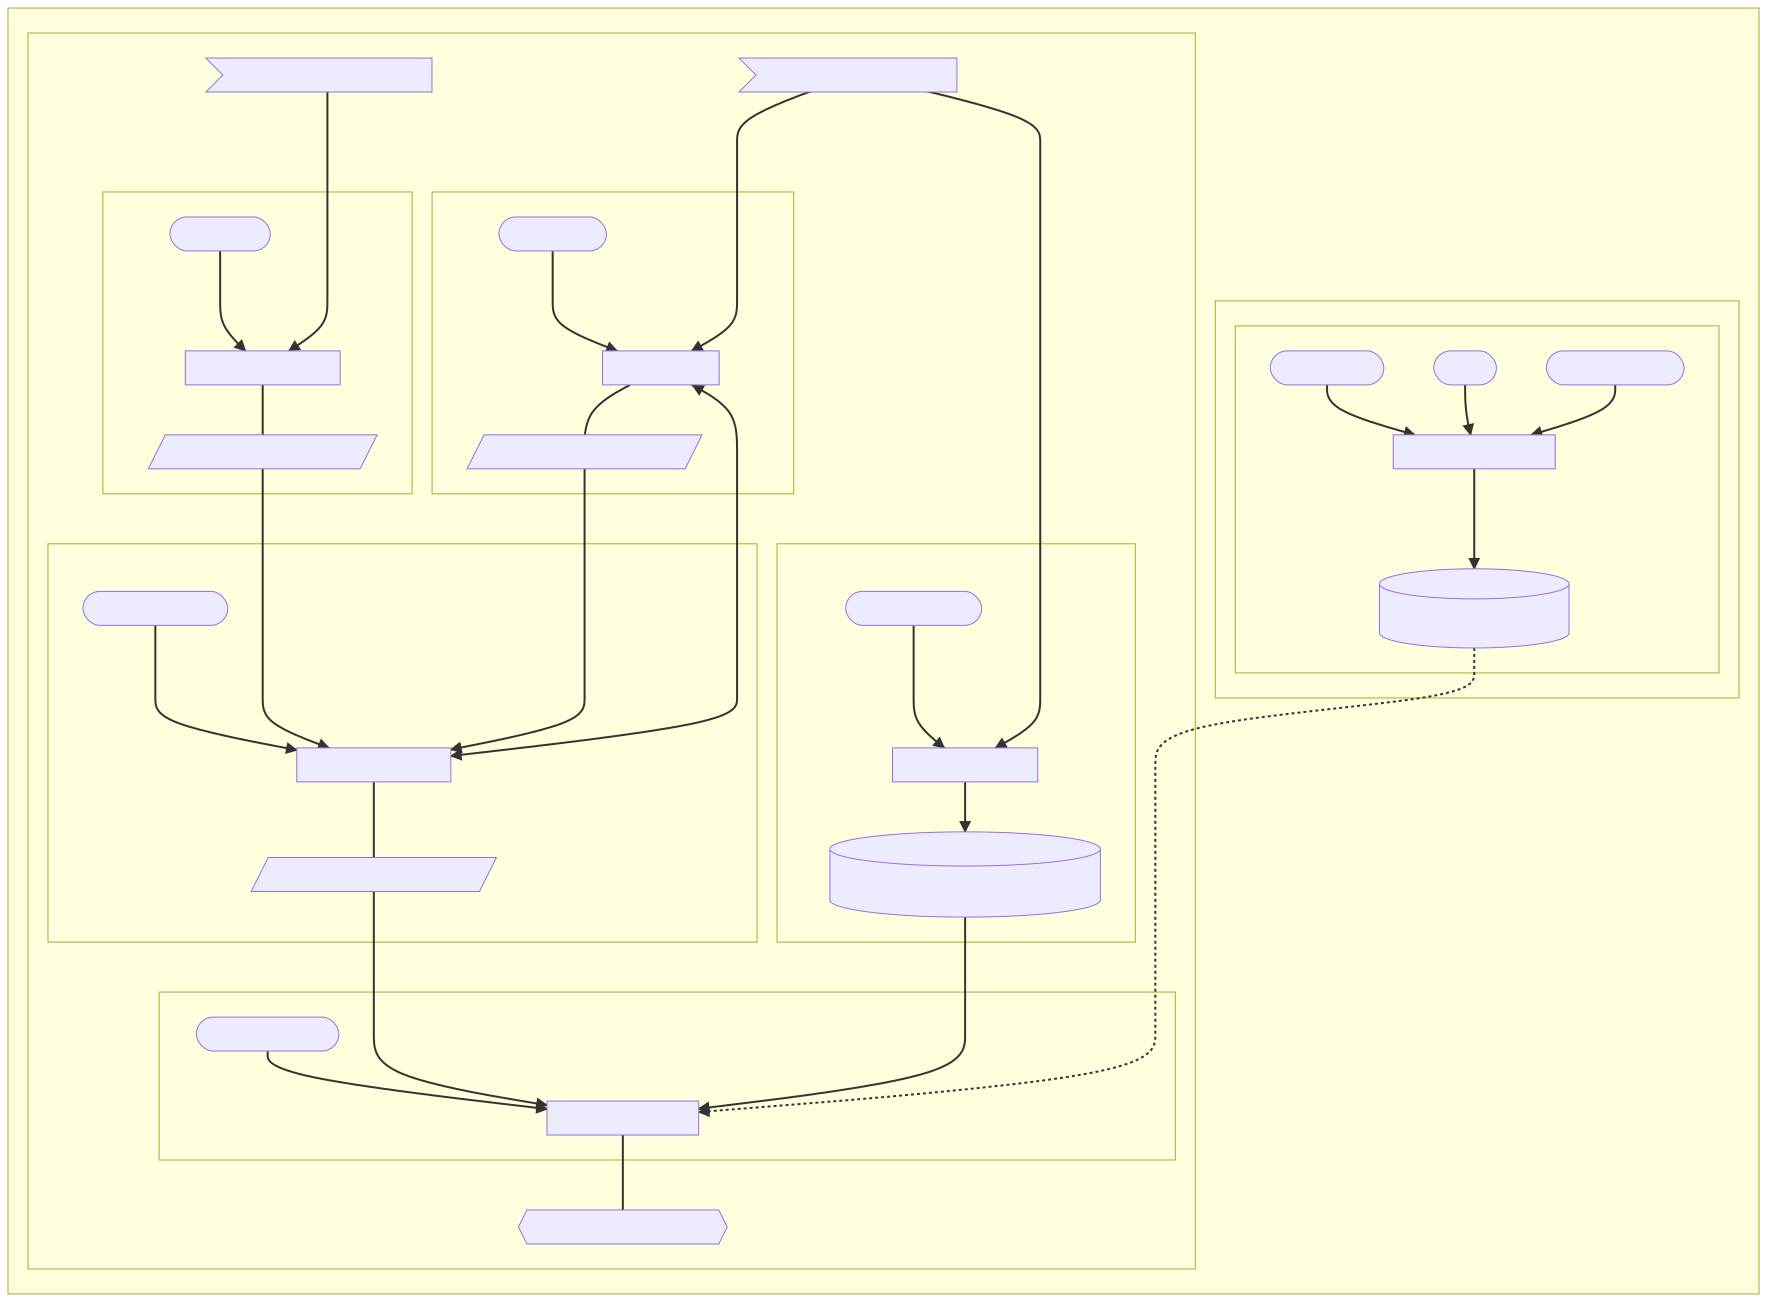
\includegraphics[width=\textwidth]{img/overview.pdf}
    \caption{High-level overview of the design proposal for our application framework.}
\end{figure}

\texttt{rt-app}'s design is based around some components considered a standard in the mobile robotics field, such as:
\begin{itemize}
    \item The \textit{pose}, which is the basic unit of data containing all of the information about the orientation and speed of a rigid object such as the mobile platform, plus timestamping.
    \item The \textit{odometry}, which constantly elaborates the data received from the mobile platform's wheel encoders, to keep track of where the robot is going.
    \item The \textit{costmap}, which is responsible for determining how likely the robot is to collide with an obstacle, using a predefined map and integrating data from other sources.
    \item The \textit{local planner}, which drives the robot towards a goal using the data provided by the odometry and various other sources, such as AMCL.
    \item \textit{AMCL}, which is an algorithm that uses data coming from the sensors, such as a LiDAR, to greatly improve the quality of the localization \cite{roswiki-amcl}.
    \item The \textit{global planner}, which builds a global plan and the costmap from raw data on startup.
\end{itemize}

Moreover, we have envisioned the following components:
\begin{itemize}
  \item The \textit{pose manager}, which is a pivotal component that manages the lifecycle of a pose, controls the flow of data between the modules, and makes sure that timestamping is consistent.
  \item The \textit{dispatcher}, which takes care of initializing threads and setting up shared memory, and is responsible for terminating the application once all workers have finished their job.
\end{itemize}

Most of these operations are performed \textit{on-line}, as their support threads will be scheduled in a real-time environment, except for global planning and thread dispatching, both of which happen once when the execution starts.

\subsection{Kernel}

An integral part of our design revolves around exploiting the capabilities of a real-time operating system: in the Linux world, this can be accomplished through co-kernel solutions, like Xenomai or RTAI, or via the \texttt{PREEMPT\_RT} patch.

The \texttt{PREEMPT\_RT} patch was introduced in 2005 to reduce the latency and increase the determinism of the Linux kernel. Since its inception, it has slowly gained traction amongst the kernel developers' community, and it's hopefully going to be merged into mainline soon \cite{lwn-rt-future}. Given that the co-kernel approach requires an application to use custom APIs, we've chosen to patch our kernel: this ensures that any program written and compiled on off-the-shelf Linux distributions will run unmodified on a patched kernel and benefit from it.

The goal of the patch is not to make the system faster but rather to eliminate virtually all of the mechanisms that introduce unbounded latencies in kernel space. By doing this, the RT kernel can improve the consistency of the system calls significantly \cite{dmoceri-benchmarking-rtlinux}, albeit with a moderate performance hit. A formal model of the Linux kernel latencies and a tool to analyze them have been developed by \textcite{demistifying-rt-latency}.

Nowadays, the impact of \texttt{PREEMPT\_RT} may not be immediately obvious, as many of its features have trickled down from the patch to the mainline kernels over the last 16 years; the most notable examples, from an academic standpoint, are:

\begin{itemize}
    \item The \textit{priority inheritance} system, which attempts to solve the well-discussed \cite{buttazzo-hard-rt} problem of priority inversion by temporarily boosting the priority of a low priority thread that shares a lock with a higher priority one until it's out of the critical section.
    \item The introduction of \textit{threaded interrupt handlers}, which are necessary to reduce unbounded latencies associated with non-deterministic peripherals such as Human Interface Devices (HIDs, e.g. a mouse) and network interfaces.
\end{itemize}

The threaded interrupt handling system, specifically, is quite beneficial to RT performance: by splitting the Interrupt Service Routine (ISR) into a small portion of code that swiftly copies the data from the peripheral's buffer registers to the kernel memory and marks the entry point of the second, beefier, one for scheduling in a kernel thread, the threaded ISR architecture ensures that an interrupt will not preempt and potentially block for a substantial time a running high-priority user thread. Once it gets green-lighted by the scheduler, the second portion of the ISR will perform all of the housekeeping necessary to present the data from the serviced peripheral to the applications through the kernel APIs.

However, a small portion of the improvements and most configuration options offered by the patch still elude the mainline: this is why to appreciate its benefits, the kernel must be patched, reconfigured, and rebuilt from source. While this operation is straightforward, it can also be very time-consuming, as fully rebuilding a kernel on commodity hardware may take several hours.

A thorough analysis of the topics we've briefly covered over this section has been performed by \textcite{survey-preempt-rt}, and it's been instrumental in understanding the extent of the \texttt{PREEMPT\_RT} patch, while practical tests which yielded rather disappointing results are described in \autoref{appendix:rt-test-lat}.

\subsection{Scheduler}

The other fundamental part of a real-time system is the scheduler: since kernel 2.6.22, when the Completely Fair Scheduler (CFS) replaced the older O(1) algorithm as the default scheduler \cite{lwn-cfs-merge}, Linux offers a complex and modular scheduling system based on several independent priority classes. 

\begin{figure}[H]
    \centering
    \includegraphics[width=\textwidth]{img/sched-class.pdf}
    \caption{The relationship between the scheduling classes provided by the Linux kernel}
\end{figure}

In each priority class, there may be several different \textit{scheduling policies} that a programmer or a system administrator might choose for a specific workload; briefly: 

\begin{itemize}
    \item \texttt{STOP}: This is the highest priority class, and it's used in kernel space to pin portions of code on specific cores in an SMP setting.
    \item \texttt{DEADLINE}: This class is mostly used to schedule periodic tasks with an EDF algorithm, which is well suited to real-time workloads, such as video decoding and real-time process control.
    \item \texttt{RT}: This is a POSIX standard compatible scheduling class that is used for some latency-sensitive tasks.
    \item \texttt{CFS}: This is the class that's commonly used for all the processes in userspace, and it's the one that uses the \texttt{nice}ness mechanism.
    \item \texttt{IDLE}: This class is responsible for keeping a CPU idling when there are no schedulable tasks left in any queue.
\end{itemize}

For a more detailed description of the scheduling classes, refer to \texttt{sched(7)} \cite{man-sched-7}.

\subsubsection{The \texttt{SCHED\_DEADLINE} scheduling policy}

%% brief history of sched-edf and who's behind it
\texttt{DEADLINE} is a scheduler developed by Dario Faggioli et al. \cite{lwn-faggioli-mail} that's been available in Linux since kernel 3.14 \cite{kn-linux-314}. This scheduler allows the programmer to define and schedule tasks using an Earliest Deadline First (EDF) algorithm, combined with a mechanism called Constant Bandwidth Server (CBS) to perform resource reservation \cite{cbs-algorithm}.

From a programming standpoint, \texttt{SCHED\_DEADLINE} exposes a rich interface to the scheduler that a developer can use to tune the behavior and constraints of a real-time task; the most significant parameters are: 

\begin{itemize}
    \item The \textit{period}, or the interval at which the scheduler will allow the task to run again after it yielded.
    \item The \textit{deadline}, or the time after which the task has taken too long to complete, and the application must take action.
    \item The \textit{runtime}, or the task's expected worst-case execution time.
\end{itemize}

The EDF algorithm is well-known in the literature for its reliability and ability to fully utilize the system's computational resources \cite{buttazzo-hard-rt}, making it ideal for our demo's purposes.

\section{Implementation}

Due to the nature and the duration of this project, implementing the whole application would have been impossible: thus, we've decided to focus on a specific subset of functionalities fundamental for a robot that needs to move and avoid obstacles autonomously. Substantially more attention was given to the research required to steer the project in the right direction and on the real-time aspects of the framework than on the actual payload: as such, the accuracy of the navigation algorithms is not exactly top-notch.

\subsection{Components}

From a software engineering standpoint, there are three distinct kinds of components:

\begin{itemize}
    \item Modules: a header and a source file that contain the schedulable units of the application. Each module contains at least an entry point function executed upon scheduling and some other functions necessary to perform specific tasks.   
    \item Helpers: headers that provide inline functions that wrap around system calls and kernel facilities in a standard way.
    \item Adapters: portions of code that provide a high-level interface to a hardware platform like Otto.
\end{itemize}

The only exceptions to this rule are the \texttt{main.c} file, which provides a scheduling facility, and the \texttt{config.h} file, which contains preprocessor definitions used to change the behavior of the application for debugging purposes.

A permanent link to the current version (as of June 2021) of \texttt{rt-app}'s codebase is available on IRALab's GitHub page \cite{rta-ira-repo}: the source code available in the repository and the documentation automatically generated from it by Doxygen are considered complementary to this report.

\subsection{Threads and scheduling}
Each module contains a schedulable unit, a portion of code that is capable of running in a separate thread, and several scheduling parameters for a \texttt{sched\_setattr()} call to modify the scheduling attributes of the associated thread.

This flexible architecture lets the programmer control how the system will schedule a specific module and by using which algorithm. When using \texttt{SCHED\_DEADLINE}, for example, the programmer can provide a \textit{deadline}, a \textit{runtime} and a \textit{period}: the scheduler will use those parameters to execute the thread appropriately and to know after which amount of time, at worst, it's expected to yield.

To change those parameters, the programmer must define a \texttt{sched\_attr} structure containing some information such as what policy to use, how to react to certain events, and parameters specific to each algorithm, such as a deadline.

\begin{listing}[H]
\inputminted[frame=single,framesep=10pt]{c}{snippets/sched-attr.c}
\caption{Example of the \texttt{sched\_attr} structure for a task with a deadline of 11ms, and a period of 20ms.}
\end{listing}

The \texttt{SCHED\_FLAG\_DL\_OVERRUN} tells the scheduler that we want it to generate a \texttt{SIGXCPU} signal when it detects a deadline miss: this is useful because we can define a recovery behavior that extends or overrides the default one.

\begin{listing}[H]
\inputminted[frame=single,framesep=10pt]{c}{snippets/dl-miss-handler.c}
\caption{Example of a deadline miss handler.}
\end{listing}

Lastly, the thread must perform a \texttt{sched\_setattr()} call to tell the scheduler that we want to use different scheduling parameters than the default ones: if the user running the program has the appropriate rights and no errors occur, the kernel will migrate the task to \texttt{DEADLINE}'s ready queue for execution.

\begin{listing}[H]
\inputminted[frame=single,framesep=10pt]{c}{snippets/entry-point.c}
\caption{Example of a periodic task scheduled with \texttt{SCHED\_DEADLINE}.}
\end{listing}

%https://lwn.net/Articles/743946/

\subsection{Timing}

As usual in systems interacting with hardware sensors, timing is a critical part of our demonstration: a simple timekeeping system, wrapping the \texttt{clock\_*()} family of system calls, has been implemented to readily provide information such as global time deltas in nanoseconds that are useful for timestamping information coming from the adapters. This collection of inline functions and globals is a helper and resides in the \texttt{h\_time.h} header. 

Besides keeping a time base and calculating deltas, the helper mostly performs conversions: since the standard library uses \texttt{timespec} structures to pass values around, \texttt{h\_time} is also responsible for translating \texttt{timespec}s to nanoseconds where needed.

\begin{listing}[H]
\inputminted[frame=single,framesep=10pt]{c}{snippets/time.c}
\caption{Example demonstrating the usage of \texttt{clock\_gettime()}, and the conversion of a \texttt{timespec} structure to nanoseconds.}
\end{listing}

\subsubsection{Obtaining a reliable time source}

The x86\_64 (AMD64) architecture provides access to a series of hardware clocks via the \texttt{RDTSC} and \texttt{RDTSCP} instructions, which the operating system can use to keep track of the time. These instructions allow the kernel to query the \texttt{TSC} (Time Stamp Counter) internal register to provide us with a reliable hardware time source. However, Intel introduced the \texttt{TSC} register back in the days of the Pentium architecture, and with the advent of technologies like out-of-order execution, hibernation, and multi-core processing, it is not advisable to solely rely on it anymore. This problem, and several possible solutions, have been discussed both in official documentation \cite{intel-rdtsc-bench} and articles from notable sources \cite{ms-rdtsc-issues}.

Conveniently, the Linux kernel works around this problem for us: to accurately advance its internal timers, the kernel uses several clock sources and a unit of measurement called \textit{jiffy}, which is tied to the value of \texttt{HZ} and is fine-tuned to each architecture's needs \cite{elinux-hrts}. Thanks to this complex architecture, which is described in depth by the manual pages \cite{man-clock-getres-2}, we can trust the values provided by system calls such as \texttt{clock\_gettime()} because they're consistent enough to give us usable values in the tens of nanoseconds range.

\subsection{Logging}

The problem of logging arose while trying to debug an issue we had with the USAD mobile platform earlier this year: the system experienced a crash, and we were not able to pinpoint a cause because the navigation stack did not use the logging facilities provided by the operating system. For this reason, it would've been difficult to precisely determine when a specific error happened in the time domain of the whole system, even if the crash didn't wipe the application logs completely.

To solve this problem, we've decided to use \texttt{syslog()}, which is the standard way to implement logging in Linux: this facility is well documented and offers better performance compared to \texttt{printf()} since there's no data actively written to the console. It should be noted that \texttt{syslog()} does still perform a blocking call by making a \texttt{write()} call to the log specified by the programmer: a potential solution to this issue could be Facebook's \texttt{liblogfaf} \cite{fb-liblogfaf}, but the project has been long since discontinued.

\begin{listing}[H]
\inputminted[frame=single,framesep=10pt]{c}{snippets/syslog-example.c}
\caption{Example demonstrating how a program might use \texttt{syslog()} to push warning messages to the global system log.}
\end{listing}

By far, the true benefit of using \texttt{syslog()} lies in the design of the Linux logging system itself: everything that's written to \texttt{/var/log/syslog} has a timestamp and, when the file reaches a set size, the logging daemon backs up the old data for later analysis before overwriting it, and powerful tools like \texttt{journalctl} let a system administrator interactively sift through the logs even if recovered from a local or remote backup.

\begin{figure}[H]
    \centering
    \includegraphics[width=\textwidth]{img/journalctl.png}
    \caption{Demonstration of the usage of \texttt{journalctl} for log analysis.}
\end{figure}

\subsection{Communications}

As we stated earlier, the \textit{adapters} provide a clean way to interact with various peripherals: an adapter is essentially an implementation of a standard interface between a module and a device driver that wraps around the lengthy set-up portion and system calls a programmer would use to access the hardware.

\subsubsection{Communicating with the Otto mobile platform}

Presently, the demo application issues command to the Otto mobile platform via an FTDI UART using serial communications. The \texttt{a\_otto} adapter provides functions that wrap around the \texttt{read()} and \texttt{write()} system calls to communicate with Otto's STM32 microcontroller over the serial line. All the data passed through the serial port is encoded and decoded using the NanoPB library, an implementation of Google's Protocol Buffers. A detailed description of Otto's communication protocol and its original implementation has been given by \textcite{fdila-bs-otto}.

Getting serial communications to work reliably with our setup was problematic: it's difficult, given Otto's current design, to synchronize the computer and the microcontroller in a way that guarantees us that data will pass through the serial port while the Odometry module's thread is executing. Using a blocking \texttt{read()} could potentially solve this problem, but it would introduce an unbounded latency: for some reason we were not able to determine, the call could block for an indefinite amount of time, triggering a deadline miss and disrupting the outgoing flow of poses.

The most commonly adopted solution in similar cases seems to be running \texttt{read()} with a timeout in a loop, catching data until the desired amount is reached. This is not desirable in our case because it would take an arbitrary amount of time and potentially mess with the alignment of the messages, rendering them difficult or downright impossible to decode. 

The workaround we employed for this issue is using a non-blocking call in combination with double buffering: this allows us to receive an arbitrary amount of data from the serial port without blocking the Odometry and detect whether or not the whole message, which is 20 bytes in length, has been received from Otto. In our loop testing, we've determined that a delay is likely to occur sometime after the first ten iterations and that this method is able to detect and rearrange split messages consistently, albeit sacrificing some throughput.

\begin{listing}[H]
\inputminted[frame=single,framesep=10pt]{c}{snippets/otto-buffering.c}
\caption{The buffering workaround necessary to make sure that no bytes are lost in-flight between the kernel and the Odometry algorithm.}
\end{listing}

\section{Future Development}

While a good portion of the groundwork has been completed, the demo in its current state is barely more than a proof of concept: to make it a usable product for controlling mobile platforms, aspects like the communications system needs to be improved, and some "bona fide" interfaces must be standardized.

One of the first aspects of the whole framework that need some work is the serial adapter: ideally, the communication protocol should be entirely rewritten to behave synchronously. The current logic is way too sensitive and wasteful of resources to employ in anything other than a controlled environment: as such, the control system must be adapted to request specific data from the microcontroller, which should avoid spamming the communication channel with responses.

As the results of the tests described in \autoref{appendix:rt-test-lat} seem to point out, the benefits of \texttt{PREEMPT\_RT} are unclear: this is an important issue that undermines the very foundation of our work and must be solved promptly. The issue might simply lie in the way we configured the kernel or in the algorithm we used for testing: configuration and performance measurement, in general, are complicated affairs, and they're some of the aspects of our work that need to be improved upon the most.

The most critical parts, instead, that we've yet to define are a module to track the creation of threads, which is currently done rather crudely in \texttt{main()}, and a standard mechanism for inter-module communication, which is probably one of the most fundamental aspects of such a system.

Some other ideas that we've not been able to pursue, but are definitely less urgent, are:

\begin{itemize}
    \item The possibility of adding adapters that work on network sockets instead of hardware devices, to extend the framework to a multi-node scenario;
    \item The development of a benchmark for inter-thread communication primitives that would let us measure the impact of each locking mechanism (semaphores, mutexes, pipes, et cetera) on latency and processing time.
\end{itemize}

Implementing those features would open up a lot of possibilities for tweaking and improving the demo package, and will be placed down the roadmap for future work.

\newpage
% Ch3
\appendix
\chapter{Implementation Issues}

While developing this demo, we have encountered some issues that, while not integral to the purpose of this document, have had a notable impact on the design and implementation process of the application: this appendix briefly summarizes them.

\section{Emulating the mobile platform}

Due to the logistic nightmare caused by the COVID-19 pandemic, the IRAlab team has not been able to source the necessary components to fix the Otto mobile platform for several months. This delay posed a serious problem since the adapter for Otto is required by the Odometry, making it hard to design and test the module.

To work around this problem, we've set out to simulate Otto's communication stack by using an ESP8266 microcontroller and UART on a NodeMCU "amica" 1.0 development board to provide dummy data to the demo's Odometry module for testing. 

While we've tried to follow Otto's specification as closely as possible, and this meant that we could work on integrating the NanoPB library in our code, we could not iron out all the differences: this eventually caused a deluge of issues since the behavior of the STM32 microcontroller was slightly more complex, and making it work reliably was a major setback.

Essentially, the STM32's reset line was hooked up to the \texttt{DTR} pin of the UART to make it possible to reset the control board when starting up the application: this was done in the ROSPy node responsible for controlling Otto by changing the value of the \texttt{dtr} member of the \texttt{Serial} object. In Linux, this process is more involved and requires issuing a specific \texttt{ioctl()} system call: for unclear reasons, this would not work on our system and, due to a programming oversight, it would fail silently.  Upon discovering the issue, we could not find a solution in software, and we ultimately resorted to decoupling the STM32's reset ping from the UART and manually resetting the board whenever needed.

\section{Measuring the average latency of the system}\label{appendix:rt-test-lat}

To measure the performance of our timing system, we've developed a small test suite: exploiting the same design used for the Odometry module, a thread performing 100 die rolls is scheduled with a period of 20ms and a deadline of 11ms. At first, we used \texttt{RDRAND}, which takes a fair amount of clock cycles,  to simulate the die rolls, but the lack of said instruction on Intel Core processors based on the Sandy Bridge (2nd gen) architecture forced us to go back to a more traditional, but less intensive, \texttt{srand()}/\texttt{rand()} approach.

Before each die-rolling cycle, the \texttt{CLOCK\_MONOTONIC} timer is queried with the method described above: this gives us a fair idea of how much skew there is between the expected 20ms interval between each iteration and the time it took the kernel to run our code.

\begin{listing}[H]
\inputminted[frame=single,framesep=10pt]{c}{snippets/latency-test.c}
\caption{By running this payload with a specific scheduler, useful data about the average jitter in different conditions can be gathered.}
\end{listing}

Running this latency test on our Lenovo ThinkPad X220 running an Intel Core i5-2520M dual-core CPU at 2.50GHz with SMT and power management disabled in the BIOS settings yielded less encouraging results than expected: the kernel that's been patched with \texttt{PREEMPT\_RT}, while resulting in less jitter in heavily loaded scenarios, is significantly less effective when the system is otherwise idling.

\begin{figure}[H]
    \centering
    \includegraphics[width=\textwidth]{img/vanilla-vs-rt-chart.pdf}
    \caption{Comparison of the average latency jitter with different kernels under normal circumstances vs. under heavy load, synthetically achieved by downloading and decoding a 4K video in real time from the internet.}
\end{figure}

The small perceived improvement in performance shows how difficult it is to determine the benefits of a real-time kernel and highlights the necessity of performing more tests and trying different configurations in the future.

\section{Hardware features that impact real-time performance}

\subsection{Caches}

Most, if not all, modern microarchitecture designs employ a multilayered cache architecture to reduce data access times significantly: while having big static RAM chips is not economically viable, relatively small-sized ones such as the caches allow chip designers to boost performance significantly for a moderate cost.

However, for the real-time application developer, cache memory is a necessary evil: while disabling it would cripple the processor, the presence of miss penalties means that performing static timing analysis on real-time code running on a modern x86 processor can be complicated.

\subsection{Symmetrical Multiprocessing}

Symmetrical Multiprocessing (SMP) is a common practice in modern computing systems: most microprocessors and even some microcontrollers contain several copies of themselves, called "cores" that work in parallel to enhance the processing power of the system. This enhancement, however, does not come for free: the programmer must be careful to avoid race conditions, situations where separate program flows could affect each other by accessing the same memory location without obeying specific constraints, such as timing or ordering. 

Since race conditions can lead to potentially catastrophic results, such as program errors or stalls, and are very hard to control, MP-enabled operating systems are designed to give the programmer as little control as possible on critical jobs such as scheduling and synchronization: by providing high-level abstractions to the underlying hardware, such as semaphores, mutexes, and threads the kernel ensures that no rogue userspace process can jeopardize the whole system.

Furthermore, the idea of using SMP in real-time environments poses an interesting problem: while it's known that the impact of processing power scaling is not linear in a classic workload, it might even be detrimental to the performance of some RT scheduling algorithms \cite[pp.~42-51]{buttazzo-hard-rt}.

\comment{ \todo{EDF sched test for MP not enough???}}

To mitigate these issues, the Linux kernel provides several ways to manage a multiprocessor environment, such as \texttt{cpuset(7)} \cite{man-cpuset-7}, a facility used to pin specific tasks to one or more cores, or as the \texttt{isolcpus} kernel flag that forces specific cores out of the kernel's load balancer, that can be used to regulate access to processing resources.

Despite all of its drawbacks and potential pitfalls, multiprocessing is still one of the most viable ways to increase the computational power of a single chip, since breaking the 4GHz barrier has proven rather arduous \cite{p4-failure}, and no modern operating system can avoid taking advantage of MP environments.

\subsection{Other facilities}

Other facilities like Simultaneous Multithreading (SMT) and power management may introduce non-determinism due to their design and operating principles: pipelining instructions from multiple threads and dynamically scaling the system clock to save power are effective techniques to maximize the use of system resources in an interactive or batch workflow, but their impact on real-time scenarios is hard to quantify.

However, running the test described in \autoref{appendix:rt-test-lat} with different BIOS configurations yielded noteworthy results: the most substantial improvement comes from disabling SMT, which results in a fourfold decrease in worst-case latency (from over 80000 nanoseconds, out of scale, to less than 20000) while disabling power management on top of it takes it down just a little further.

\begin{figure}[H]
    \centering
    \includegraphics[width=\textwidth]{img/smt-pm-chart.pdf}
    \caption{Latency jitter over 100 iterations of a task performing 100 \texttt{rand()} calls scheduled with \texttt{SCHED\_DEADLINE} (Period: 20ms; Runtime/WCET: 10ms; Deadline: 11ms) on Ubuntu GNU/Linux 20.04 LTS with kernel \texttt{Linux 5.8.0-53-generic \#60~20.04.1-Ubuntu SMP Thu May 6 09:52:46 UTC 2021 x86\_64} and varying BIOS configuration.}
\end{figure}

While those functionalities can regularly be disabled in the BIOS settings, there are others that the user can't control on most systems, like the Intel Management Engine (ME) and its AMD counterpart Secure Processor (AMD-SP). Those so-called "security features" are not auditable due to their secretive design thus their impact on real-time performance is unknown.

\comment{
\subsection{Filesystem and I/O performance}

While the I/O architecture of Linux has been well documented and analyzed in the literature, the impact of disk I/O, and specifically of the filesystem on application, performance has not. The lack of research material in this field can probably be attributed to the rarity of real-time disk I/O bound workloads, but it's an interesting topic nonetheless.
}

% Tail
%\addcontentsline{toc}{chapter}{Bibliography}

\printbibliography[title={References}]
%\printbibliography[nottype=online,title={Bibliography}]
%\addcontentsline{toc}{chapter}{Sitography}
%\printbibliography[type=online,title={Sitography}]

\end{document}